
\documentclass[12pt]{article}

% Layout.
\usepackage[top=1in, bottom=0.75in, left=1in, right=1in, headheight=1in, headsep=6pt]{geometry}

% Fonts.
\usepackage{mathptmx}
\usepackage[scaled=0.86]{helvet}
\renewcommand{\emph}[1]{\textsf{\textbf{#1}}}

% TiKZ.
\usepackage{tikz, pgfplots}
\usetikzlibrary{calc}
\pgfplotsset{compat = newest}
 
\pgfplotsset{my style/.append style={axis x line=middle, axis y line=
middle, xlabel={$x$}, ylabel={$y$}, axis equal }}

% Misc packages.
\usepackage{amsmath,amssymb,latexsym}
\usepackage{graphicx}
\usepackage{array}
\usepackage{xcolor}
\usepackage{multicol}

% Commands to set various header/footer components.
\makeatletter
\def\doctitle#1{\gdef\@doctitle{#1}}
\doctitle{Use {\tt\textbackslash doctitle\{MY LABEL\}}.}
\def\docdate#1{\gdef\@docdate{#1}}
\docdate{Use {\tt\textbackslash docdate\{MY DATE\}}.}
\def\doccourse#1{\gdef\@doccourse{#1}}
\let\@doccourse\@empty
\def\docscoring#1{\gdef\@docscoring{#1}}
\let\@docscoring\@empty
\def\docversion#1{\gdef\@docversion{#1}}
\let\@docversion\@empty
\makeatother

% Headers and footers layout.
\makeatletter
\usepackage{fancyhdr}
\pagestyle{fancy}
\fancyhf{} % Clears all headers/footers.
\lhead{\baselineskip 30pt
%\emph{\@doctitle\hfill\@docdate}
\emph{\@docdate\hfill\@doctitle}
\ifnum \value{page} > 1\relax\else\\
\emph{Name: \rule{3.5in}{1pt}\hfill \@docscoring}\fi}
\rfoot{\emph{\@docversion}}
\lfoot{\emph{\@doccourse}}
\cfoot{\emph{\thepage}}
\renewcommand{\headrulewidth}{0pt}%
\makeatother

% Paragraph spacing
\parindent 0pt
\parskip 6pt plus 1pt

% A problem is a section-like command. Use \problem{5} to
% start a problem worth 5 points.
\newcounter{probcount}
\newcounter{subprobcount}
\setcounter{probcount}{0}
\newcommand{\problem}[1]{%
\par
\addvspace{4pt}%
\setcounter{subprobcount}{0}%
\stepcounter{probcount}%
\makebox[0pt][r]{\emph{\arabic{probcount}.}\hskip1ex}\emph{[#1 points]}\hskip1ex}
\newcommand{\thesubproblem}{\emph{\alph{subprobcount}.}}

% Subproblems are an enumerate-like environment with a consistent
% numbering scheme. 
% Use \begin{subproblems}\item...\item...\end{subproblems}
\newenvironment{subproblems}{%
\begin{enumerate}%
\setcounter{enumi}{\value{subprobcount}}%
\renewcommand{\theenumi}{\emph{\alph{enumi}}}}%
{\setcounter{subprobcount}{\value{enumi}}\end{enumerate}}

% Blanks for answers in normal and math mode.
\newcommand{\blank}[1]{\rule{#1}{0.75pt}}
\newcommand{\mblank}[1]{\underline{\hspace{#1}}}
\def\emptybox(#1,#2){\framebox{\parbox[c][#2]{#1}{\rule{0pt}{0pt}}}}

% Misc.
\renewcommand{\d}{\displaystyle}
\newcommand{\ds}{\displaystyle}
\def\bc{\begin{center}}
\def\ec{\end{center}}
\def\be{\begin{enumerate}}
\def\ee{\end{enumerate}}


\doctitle{Math 251: Quiz 3}
\docdate{Sept 9, 2021}
\doccourse{UAF Calculus I}
\docversion{v-1}
\docscoring{\blank{0.8in} / 25}
\begin{document}
%\textbf{Please circle your instructor's name:} \hfill Leah Berman  \hfill   Jill Faudree\\

There are 25 points possible on this quiz. No aids (book, calculator, etc.)
are permitted.  {\emph{Show all work for full credit.}}

\problem{16} (4 pts each; 2 pts for answer, 2 pts for work) Evaluate the following limits. Give the most complete answer; if the limit is infinite, indicate that with $\infty$ or $-\infty.$ If a value does not exist, write DNE.\\

%\textcolor{red}{Like 2.3 \#97,98,103,125 respectively}

\begin{subproblems}
\item $\displaystyle{\lim_{ x\to 2} \frac{x^2-4}{x^2-5x+6}}$ 
\vfill

\item $\displaystyle{\lim_{ h\to 0} \frac{\frac{3}{2}-\frac{3}{2+h}}{h}}$ 
\vfill

\item \emph{Make sure to give some justification for your answer here.} $\displaystyle{\lim_{ t\to -3^+ } \frac{5+t}{t^2+3t}}$ 
\vfill

\item Given $\displaystyle{\lim_{ x \to 5} f(x) = 8}$ and $\displaystyle{\lim_{ x \to 5} g(x) = -10}$, evaluate $\displaystyle{\lim_{ x \to 5} \frac{3f(x) -x}{(g(x))^2}}.$ 
\vfill
\end{subproblems}
\newpage
%\textcolor{red}{like 2.4 \#133,135}
%\problem{4} Determine the point(s), if any, at which the function $\displaystyle{f(x)=\frac{x(x+1)}{(x+1)(e^x-4)}}$ is discontinuous.
%\vspace{2in}
\problem{4} Does the equation $x- \sin (\pi x) -3=0$  have a solution on the interval from $x=0$ to $x=5$? Use the Intermediate Value Theorem to justify your answer.
\vspace{3in}
\problem{5} Consider the graph of the function  $y=H(x)$  shown in the graph below.

\begin{center}
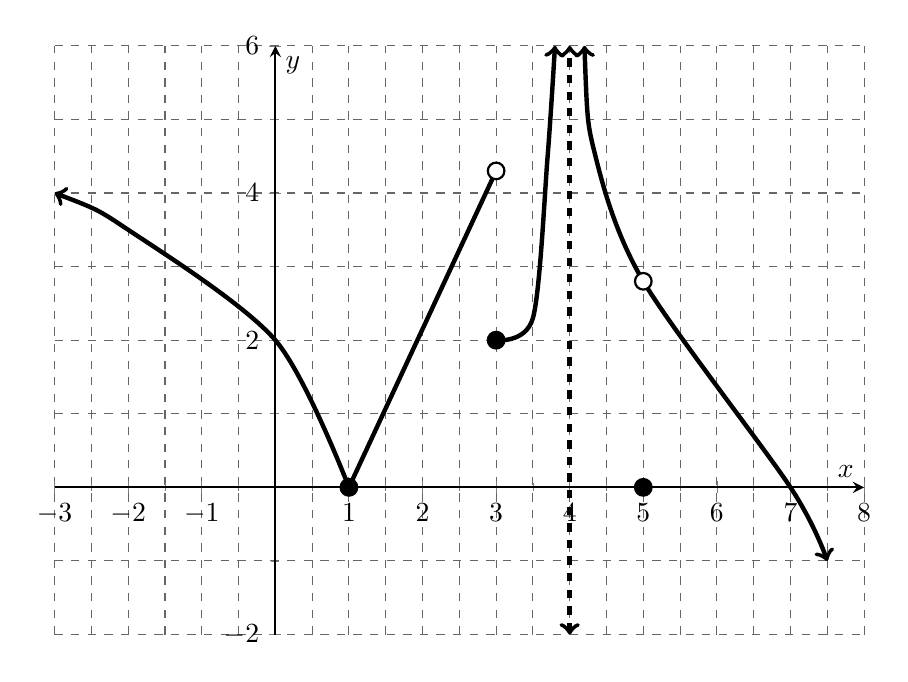
\begin{tikzpicture}
\begin{axis}[scale=1.5, thick, my style, xtick={-3,...,8}, ytick={-2, 0,...,6},
xmin=-3, xmax=8, ymin=-2, ymax=6, minor y tick num=1,
        minor x tick num=1, mark size=3.0pt, grid=both, grid style={ thin, black!60, dashed}, axis equal image]
% %%asymptote
\addplot[dashed,<->, ultra thick] coordinates {(4,-2) (4,6)};       
%%points solid
\addplot[mark=*,only marks] coordinates {(3,2)(5,0) (1,0)};
%%points open
\addplot[mark=*,fill=white,only marks] coordinates {(3,4.3)(5,2.8)};
%%Curves
\addplot[ultra thick, smooth,<-] coordinates {(-3,4) (-2,3.5) (0,2)(1,0)};
\addplot[ultra thick, smooth] coordinates {(1,0) (3,4.3)};
\addplot[ultra thick, smooth,->] coordinates {(3,2) (3.5,2.3) (3.7,4.5) (3.8,6)};
\addplot[ultra thick, smooth,<->] coordinates {(4.2,6) (4.35,4.5) (5,2.8) (7,0) (7.5,-1)};       

\end{axis}
\end{tikzpicture}
\end{center}

\begin{subproblems}
\item List all $x$-values for which the function $H(x)$ fails to be continuous.\\
\vfill
\item Label the values above as removable or nonremovable.

\end{subproblems}
\end{document}

\end{document}